\section{Software}
Softwareseitig wurde mit dem Plugin PlatformIO für Atom und Spyder für Python gearbeitet. Zur Versionierung wurde Git verwendet.
\subsection{Arduino}
Das Programm \textit{BWMvelocity.cpp} welches man in Anhang \ref{app:ardprog} findet, ermöglicht es mit Hilfe von Polling oder Interrupts die Unterbuchtszeiten der Lichtschranke zu erfassen und so auf Grund der Grösse des unterbrechenden Objekts oder auf Grund des Abstands der Lichtschranken auf die Zeit zu schliessen.

Ein Druchlauf \marg{Sensor-Signale} eines Objektes erzeugt dabei die in \ref{fig:ArdSigs} gezeigten Signale.
\begin{figure}[ht]
    \centering
    %    \missingfigure{Bild einfügen}
    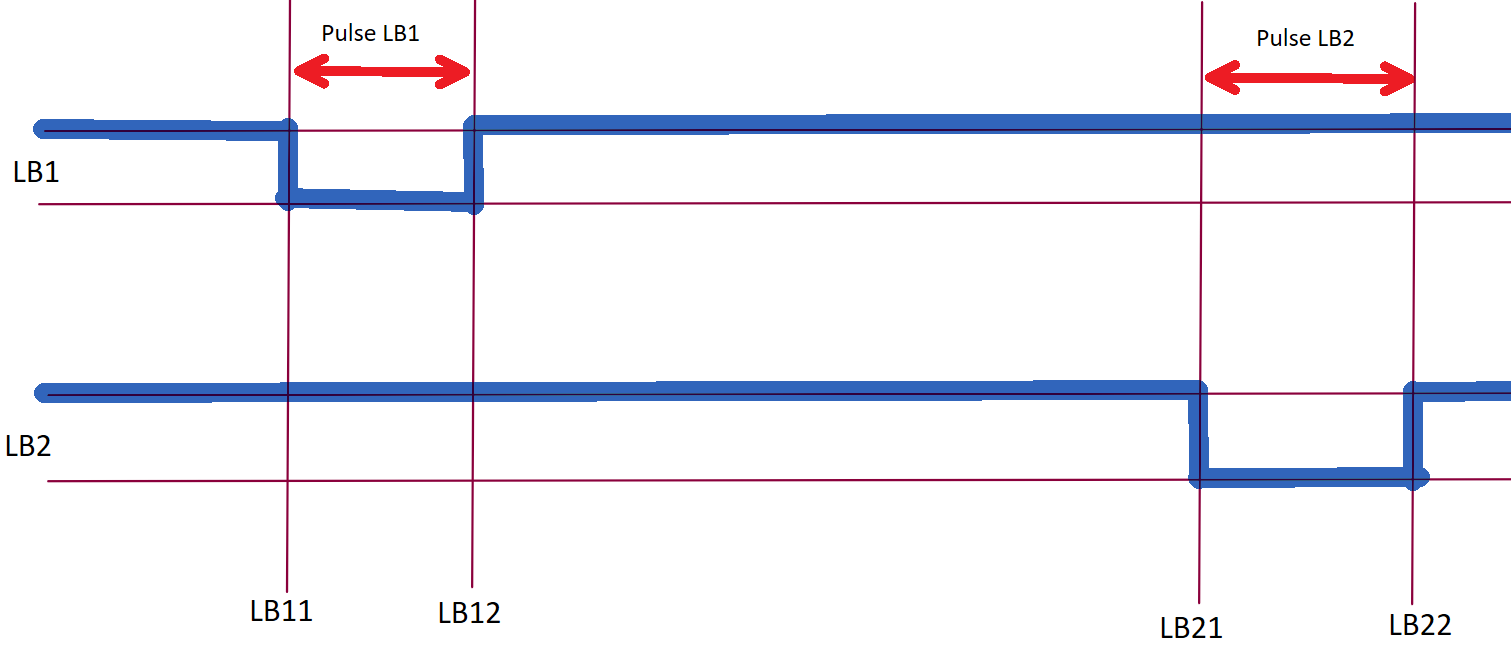
\includegraphics[width=\textwidth]{images/signals}
    \caption{Generierte Signale der Lichtschranke}
    \label{fig:ArdSigs}
\end{figure}

Der \marg{Funktionen} Code besitzt folgende Funktionen:
\begin{itemize}
    \item void setup()
    \item void loop()
    \item double calculate\_velocity\_ms(unsigned long passingduration,double distance)
    \item void printlog(double speedinkmh[4])
    \item void ISRLB1()
    \item void ISRLB2()
\end{itemize}

Weiter \marg{globale Variabeln} gibt es folgende erwähnenswerte globale Variabeln:
\begin{itemize}
    \item const double sensordistance = 101.0*1000
    \item const double ballwidth = 72.0*1000
    \item unsigned long passingtime[4]
    \item double velocitykmh[4]
\end{itemize}

Die ersten zwei beschreiben die geometrischen Randbedingungen in $\mu m$.\\
\clearpage

Das Array \textit{passingtime} beinhaltet die folgenden Einträge:\\
\begin{tabular}{lll}
    \textbf{Index}&\textbf{Zeit} & \textbf{Distanz} \\
    0&LB12 - LB11 & Ballgrösse\\
    1&LB22 - LB21 & Ballgrösse\\
    2&LB21 - LB11 & Sensorabstand\\
    3&B22 - LB12 & Sensorabstand\\
\end{tabular}\\

Das Array \textit{velocitykmh} beinhaltet die berechneten Geschwindigkeit korresponidrenden zu den Zeiten und Distanzen aus dem passingtime-Array.\\
Im Pollingmodus sind die Werte bei  Index 2 und 3 jeweils 0.

\subsubsection{Preprocessor-Direktiven}
Mit\marg{Preprocessor} Hilfe der \#define Anweisung können 3 verschiedene Modis ausgewählt werden. Dafür müssen die entsprechenden Befehle ein-kommentiert werden.\\

\begin{tabular}{L{0.3\linewidth} L{0.7\linewidth}}
    \#define MYDEBUG & Aktiviert den Debuggmodus und somit die \textit{DEBUG\_PRINT}-Funktionen.\\
    \#define MYLOG & Aktiviert den Datenloggingmodus und somit die \textit{LOG\_PRINT}-Funktionen.\\
    \#define USEINTERRUPT & Aktiviert den Interruptmodus und deaktiviert den Pollingmodus.\\
\end{tabular}

\subsubsection{Pollingmodus}
Im \marg{Polling} Pollingmodus wird mit der Funktion \textit{\href{https://www.arduino.cc/reference/en/language/functions/advanced-io/pulsein/}{pulseIn(pin, value, timeout)}} die Länge des Unterbruches in $\mu S$ angegegeben. Die minimale dedektierbare Pulslänge ist dabei 10 $\mu S$.
Es werden folgende Zeiten erfasst:\\
\begin{tabular}{ll}
    \textbf{Zeit} & \textbf{Distanz} \\
    Pulse LB1 & Ballgrösse\\
    Pulse LB2 & Ballgrösse\\
\end{tabular}

\subsubsection{Interruptmodus}
Im \marg{Interrupt}Interruptmodus wird bei jedem Flankenwechsel ein Interrupt ausgelöst und ein Zeitstempel in $\mu S$ gespeichert. Dies ergibt gesamt 4 Messwerte für LB11, LB12, LB21 und LB22. Welche im Array \textit{passingtime} abgelegt werden.\\
\\
\textbf{Beim Arduino UNO müssen die Lichtschranken dafür zwingend auf Pin 2 und 3 angeschlossen sein.}


\subsubsection{calculate\_velocity\_ms()}
\begin{center}
   Geschwindigkeit [$\nicefrac{m}{s}$] = calculate\_velocity\_ms( Zeit [$\mu S$], Distanz [$\mu m$])
\end{center}

Die Funktion \textit{double calculate\_velocity\_ms(unsigned long passingduration,double distance)} übernimmt eine Zeitdauer in $\mu S$ und eine Distanz in $\mu m$.
Sie giebt eine Geschwindigkeit in $\nicefrac{m}{s}$ zurück vom Typ double.

\clearpage
\subsubsection{printlog()}
Wenn der Datenloggingmodus aktiv ist printet die Funktion in die serielle Schnittstelle.
Im Pollingmodus:\\
\begin{tabular}{llll}
    Iteration&Bezeichnung& Puls LB1 & Puls LB2\\
\end{tabular}

Im Interruptmodus:\\
\begin{tabular}{llllll}
    Iteration&Bezeichnung& Int. LB1 & Int. LB2& Int. LB11 - LB21& Int. LB12 - LB22\\
\end{tabular}\\

\subsubsection{ISRLB1()}
Diese Funktion ist die Interrupt-Service-Routine für die Lichtschranke LB1. Sie erkennt den Signalwechsel und schreibt den aktuellen Zeitstempel LB11 oder LB12 je nach dem ob das Signal HIGH oder LOW ist. Weiter wird das Flag \textit{LBinterrupted} auf False gesetzt.\\


\subsubsection{ISRLB2()}
Diese Funktion ist die Interrupt-Service-Routine für die Lichtschranke LB1. Sie erkennt den Signalwechsel und schreibt den aktuellen Zeitstempel LB11 oder LB12 je nach dem ob das Signal HIGH oder LOW ist. Bei LB21 wird das Flag \textit{LBinterrupted} auf False gesetzt. Bei LB22 auf True. \textbf{Aus diesem Grund können die Lichtschranken nicht vertauscht werden.}\\


\subsection{Python}
Das Pythonskript aus Anhang \ref{app:python} dient dazu, die gesendeten Daten über den Serialport auszulesen und in einem .txt File abzuspeichern. Dies erleichtert die Datenanalyse mit Excel oder Matlab.